\documentclass[addpoints]{exam}

\usepackage{graphbox}
\usepackage{hyperref}
\usepackage{tabularx}
\usepackage{tikz}
\usetikzlibrary{positioning}

% Header and footer.
\pagestyle{headandfoot}
\runningheadrule
\runningfootrule
\runningheader{CS 440 Computer Graphics}{Homework 1}{Spring 2018}
\runningfooter{}{Page \thepage\ of \numpages}{}
\firstpageheader{}{}{}

\qformat{{\large\bf \thequestion. \thequestiontitle}\hfill[\totalpoints\ points]}
\boxedpoints
% \printanswers

\title{Habib University\\CS 440 Computer Graphics\\Spring 2018}
\author{Homework 1}
\date{Due: TBD}

\begin{document}
\maketitle

\begin{questions}

  \titledquestion{Mapping and Linear Interpolation}[5]
  \label{q:interpolate}
  
  \begin{tabularx}{\linewidth}{cX}
    \raisebox{-\totalheight}{
      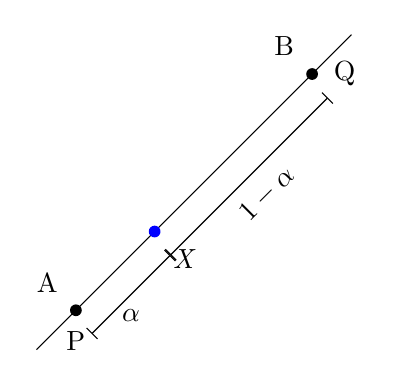
\begin{tikzpicture}
        \draw (0,0) -- (4,4);
        \node[circle,fill,inner sep=1.5pt] at (.5,.5) (P){};
        \node[circle,fill,inner sep=1.5pt] at (3.5,3.5) (Q) {};
        \node[circle,fill,blue,inner sep=1.5pt] at (1.5,1.5) (X) {};
        \node[below  = 2pt of P]{P};
        \node[right = 2pt of Q]{Q};
        \node[below right = 2pt of X]{\it X};
        \node[above left = 2pt of P]{A};
        \node[above left = 2pt of Q]{B};

        \draw[|-|] (0.7,0.2) -- node[midway,below=2pt]{$\alpha$}(1.7,1.2);
        \draw[|-|] (1.7,1.2) -- node[midway,sloped,below=2pt]{$1-\alpha$}(3.7,3.2);
      \end{tikzpicture}
    }
    &
    For any point $X$ on the line segment PQ, the distance of $R$ to the endpoints can be expressed as
    \[
      |PX| : |XQ| = \alpha:(1-\alpha)\;,\; 0 \leq \alpha \leq 1
    \]
    which leads to
    \[
      X = \alpha Q + (1-\alpha) P
    \]
    $X$ is thus said to be an \href{https://en.wikipedia.org/wiki/Affine_combination}{\it affine combination} of P and Q.
    
    Imagine a mapping from the range PQ to a new range, AB. We are interested in finding the coordinates of $X'$ which is the mapping of $X$ to the new range. Write a function {\tt map\_point(px, py, qx, qy, ax, ay, bx, by, x, y, \&\_x, \&\_y)} that takes as argument the coordinates of P, Q, A, B, and X and sets the last 2 arguments to the coorindates of $X'$.
  \end{tabularx}
  \underline{File}: {\tt interpolate.cpp}
  
  \titledquestion{Interaction: Polygons Galore}[20]
  \label{q:galore}
  
  \begin{tabularx}{\linewidth}{lX}
    \raisebox{-.9\totalheight}{\includegraphics[width=.35\textwidth]{galore}}
    &
    Write a program that interactively draws triangles and quadrilaterals. The program draws a point at the location of each mouse click. It supports two {\it modes} -- triangle mode (default) and quad mode. When in triangle mode, every 3 consecutive points are drawn as a triangle. When in quad mode, every 4 consecutive points are drawn as a quad.

    Furthermore, the following interaction is supported.\newline
    -- Pressing q or Q closes the window and ends the program.\newline
    -- Pressing r or R clears the screen and resets to default.\newline
    -- Pressing t or T toggles between the drawing modes.
  \end{tabularx}
  \underline{File}: {\tt galore.cpp}\\
  \underline{Useful functions}: {\tt \href{https://www.opengl.org/resources/libraries/glut/spec3/node49.html#SECTION00084000000000000000}{glutKeyboardFunc}, \hyperref[q:galore]{map\_point}}

  \titledquestion{Vertex Arrays: All At Once}[10]

  In Problem \ref{q:galore}, you specified the vertices one by one. Using \href{http://www.informit.com/articles/article.aspx?p=1377833&seqNum=6}{\it vertex arrays}, it is possible to specify the points all at once. Copy the file from the previous problem and modify only its display callback function (and any functions it may be calling) to use vertex arrays.
  
  \noindent\underline{File}: {\tt atonce.cpp}\\
  \underline{Useful functions}: {\tt \href{https://www.khronos.org/registry/OpenGL-Refpages/gl2.1/xhtml/glVertexPointer.xml}{glVertexPointer}}\\
  \underline{Useful links}: {\tt \href{http://www.songho.ca/opengl/gl_vertexarray.html}{Vertex Array}}\\
  
  \titledquestion{Timing: Catch Me If You Can}[20]
  We want to test our reflexes by seeing how quickly we can click on an object on screen. Write a program that displays a 2D object with non-zero area anywhere in the window. The catch is that it is going to disappear and reappear at some other location after a random time interval. You have to click on it before it disappears. If you succeed, you get 1 point. If the object has moved away by the time you clicked, you get -1. The game ends when your score becomes -3.

  \noindent\underline{File}: {catch.cpp}\\
  \underline{Useful functions}: {\tt \href{https://www.opengl.org/resources/libraries/glut/spec3/node64.html#SECTION000819000000000000000}{glutTimerFunc}}

  \titledquestion{Color Interpolation: In Memory of Tim}[5]
  \label{q:maxwell}
  
  \begin{tabularx}{\linewidth}{cX}
    \raisebox{-\totalheight}{\includegraphics[width=.35\linewidth]{maxwell}}
    &
    \href{https://en.wikipedia.org/wiki/James_Clerk_Maxwell}{James Clerk Maxwell} is best known for his work in elctromagnetic radiation resulting in the well known \href{https://en.wikipedia.org/wiki/Maxwell\%27s_equations}{Maxwell's equations}.
    
      Not surprisingly, he was also among the first ones to expore the \href{https://spie.org/publications/pm105_32_maxwell_triangle?SSO=1}{trichromatic theory of color}. This has led to what is now known as \href{http://www.appstate.edu/~steelekm/classes/psy3215/Maxwell.htm}{Maxwell's triangle}, also called simply the \href{https://en.wikipedia.org/wiki/Color_triangle}{color triangle}.
      
      The color triangle has the primary colors at its vertices and the interior is shaded by linear combinations of the colors at the vertices. At any interior point, the amount of color contibuted by a vertex is proportional to the distance of the vertex from that point.
      
      Write a program to display Maxwell's triangle.
  \end{tabularx}
  \underline{File}: {maxwell.cpp}\\
  \underline{Fun fact}: {Maxwell had a short stint at \href{https://www.abdn.ac.uk/museums/collections/james-clerk-maxwell-professor-and-physicist-457.php}{University of Aberdeen}.}\\
  
  \titledquestion{Color Interpolation}[20]

  \begin{center}
    \includegraphics[width=\linewidth]{barbw}\\
    \vspace{-75pt}\includegraphics[width=\linewidth]{barrgb}
  \end{center}

  \vspace{-25pt}In Problem \ref{q:maxwell}, we used the API's native color interpolation. For this problem, we will draw color bars for which we will perform the interpolation ourselves. We can use the technique from Problem \ref{q:interpolate} for the purpose. In later assignments we will see how to interpolate between more than 2 values as was done by the API in the above problem.
  \begin{parts}
    \part Draw a color bar that is white at one end and black at the other.
    \part Draw a color bar that is red at one end, green in the middle, and blue at the other end.
  \end{parts}
  We should be able to switch between the two color bars by commenting and uncommenting at most a couple of lines in the display callback function.
  
  \noindent\underline{File}: {colorbar.cpp}\\
  \underline{Fun Fact}: {Maxwell had a short stint at \href{https://www.abdn.ac.uk/museums/collections/james-clerk-maxwell-professor-and-physicist-457.php}{University of Aberdeen}.}
  
  \titledquestion{Approximating a Smooth Surface: $\lim\limits_{n\rightarrow\infty} \diamond = \circ$}[20]
  \begin{center}
    \includegraphics[width=\linewidth]{circle}
  \end{center}

  \begin{tabularx}{\linewidth}{lX}

    \raisebox{-\totalheight}{
  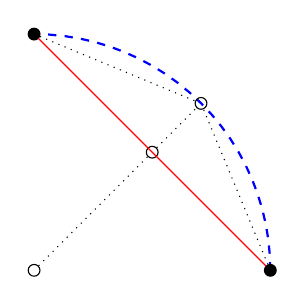
\begin{tikzpicture}
   \draw [blue,thick,dashed,domain=0:90] plot ({3*cos(\x)}, {3*sin(\x)});    
   node[circle,fill]{}(
   \node [draw,circle,fill,inner sep=1.5pt] at (0,3) (a){};
   \node [draw,circle,fill,inner sep=1.5pt] at (3,0) (b){};
   \node [draw,circle,inner sep=1.5pt] at (0,0) (c){};
   \node [draw,circle,inner sep=1.5pt] at (1.5,1.5) (p){};
   \node [draw,circle,inner sep=1.5pt] at (2.12,2.12) (q){};

   \draw [red] (a) -- (b);
   \draw [dotted] (c) -- (p);
   \draw [dotted] (p) -- (q);
   \draw [dotted] (a) -- (q);
   \draw [dotted] (b) -- (q);
 \end{tikzpicture}
 }
    &
    This problem explores the approximation of a smooth shape by a many sided polygon. Starting from a diamond on the left in the above figure, each next shape is recursively generated by inserting edge midpoints into the shape and projecting the new points to the circumference of the circle being approximated. This is illustrated in the figure on the left. The black line is approximating the blue circle. Its midpoint, when inserted, is projected to the circumfernce of the circle with respect to the circle's center.

    Generate the above figure by repetitively refining a coarse initial approximation.
  \end{tabularx}
  
  \underline{File}: {circle.cpp}
  
  \titledquestion{Triangle in a Triangle in a Triangle ...}[20]
  Sierpinski gasket.

  \titledquestion{Deja Vu}[35]
  Mandelbrot set.


  
  
\end{questions}

\end{document}



